\documentclass[twoside]{supsistudent} 


\setlength{\parindent}{0pt}

\usepackage{url}
\usepackage{listings}
\usepackage{float}% If comment this, figure moves to Page 2

% Crea un capitolo senza numerazione che pero` appare nell'indice %
\newcommand{\problemchapter}[1]{%
  \chapter*{#1}%
  \addcontentsline{toc}{chapter}{#1}%
\markboth{#1}{#1}
}

% Numerazione delle appendici secondo norma
\addto\appendix{
\renewcommand{\thesection}{\Alph{chapter}.\arabic{section}}
\renewcommand{\thesubsection}{\thesection.\arabic{subsection}}}

\setcounter{secnumdepth}{5} 	%per avere più livelli nei titoli
\setcounter{tocdepth}{5}		%per avere più livelli nell'indice


\titolo{Full-Stack Web Development with React Specialization (Hong Kong University)}
\studente{Olmo Barberis}
\modulo{HK\_Seminar}

\begin{document}

\pagenumbering{alph}
\maketitle
\onehalfspacing
\frontmatter


\pagenumbering{roman}

\newpage
\mainmatter
\pagenumbering{arabic}
\setcounter{page}{1}



The purpose of this document is to provide an overview of all the topics covered during the \textit{Full-Stack Web Development with React Specialization} on \textit{Coursera}\footnote{https://www.coursera.org/specializations/full-stack-react}. The original course is composed of four parts, but the \textit{HK\_Seminar} will cover only two parts: an introduction to React, a front-end framework for developing single-page web applications, and server-side development with NodeJS, Express, and MongoDB.

\section*{Front-End Web Development with React}

This course provide an introduction to the React framework, its components and some basic elements like routing, forms and animations. Shared state management, with the corresponding tools like Redux, is another important topic covered alongside fetching data.

\subsection*{Single Page Application}
A traditional website is a collection of pages and resources that are fetched to the server for each page that is navigated. Even if a lot of pages have part i common, like footer or header, they are requested entirely every time a new page is navigated. In a Single Page Application (SPA) the entire website is downloaded at first, then only the data that changes are re-downloaded from the server. A SPA enable to deliver a user experience closer to a desktop application, does not need to be entirely reloaded and allows the browser to re-render only the parts that are changed. 
Some downside of a SPA is that Search Engine Optmiziation (SEO) is more difficult to achieve and the initial page load can be slower than a traditional website.


\subsection*{React Overview}

React is a JavaScript library for building component-based user interfaces using a declarative approach. React focuses only on user interface and is designed for speed, simplicity and scalability.

A React component is a JavaScript class or function that  is imported from the React Module. It is then rendered using the React's rendering function \texttt{ReactCOM.render(...)}.

\subsubsection*{Components}
A component is an indipendent and reusable set of React elements that should appear on screen. Every component can accepts any input and is composed of React tags, that always start with a capital letter, and native tags, which start with lowercase letters and are treated as DOM tags.
Every component has a local state which can hold multiple information that can be passed to children components using \texttt{props}. The state is an immutable object that can be updated using the \texttt{setState(...)} directive. This function accept the property to update and merge it with the actual state. Only class components can have a local state. The state must never be manipulated directly.

Handling event is possible in a similar way as on DOM elements:

\begin{figure}[h]
    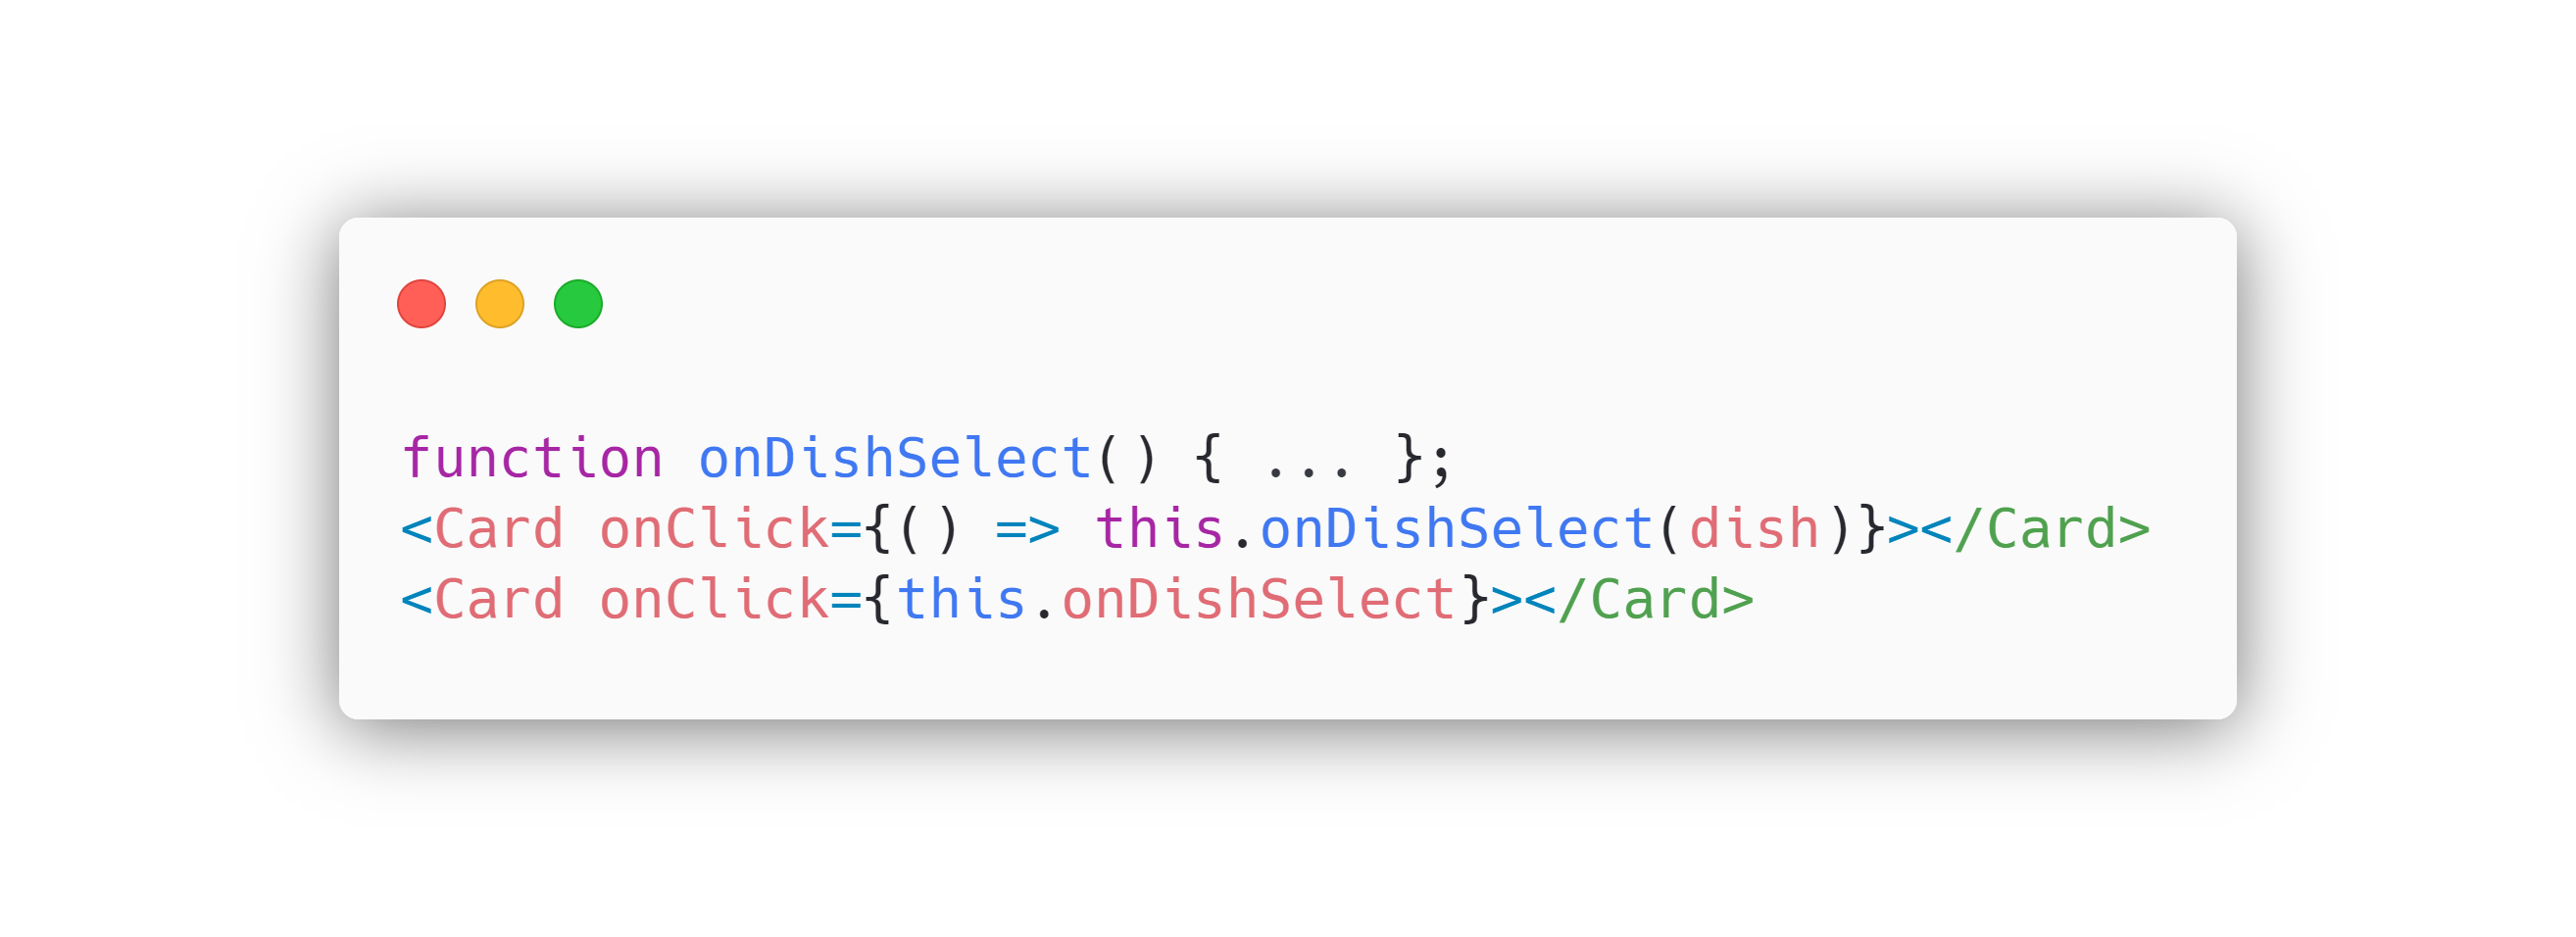
\includegraphics[width=\textwidth]{assets/react-event-handling.png}
    \caption{Event handling when clicking on div}
    \label{fig:event-handling}
\end{figure}

In Figure \ref{fig:event-handling} is possible to see how map a function to a click event on the React element \texttt{Card}.

\subsubsection*{Lifecycle}
React provides life cycle hooks/methods that can be invoked to perform certain operations. Component is created and then mounted in the application and when it's not required anymore is unmounted. There are three stages of lifecycle: mounting, updating and unmounting. Each stage provide, when component is declared as class, several methods like a construcor (mounting), \texttt{componentDidMount()} (called after mounting is finished), \texttt{render()} (call when rendering UI) and many others.

\subsubsection*{Functonal vs Class}
Until the release of \texttt{React 16.8} in 2018 there were two ways of declaring a component: class component or functional component. Functional components are s JavaScript function that returns a React element, can receive props but cannot provide local state or lifecycle hooks. 
\begin{figure}
    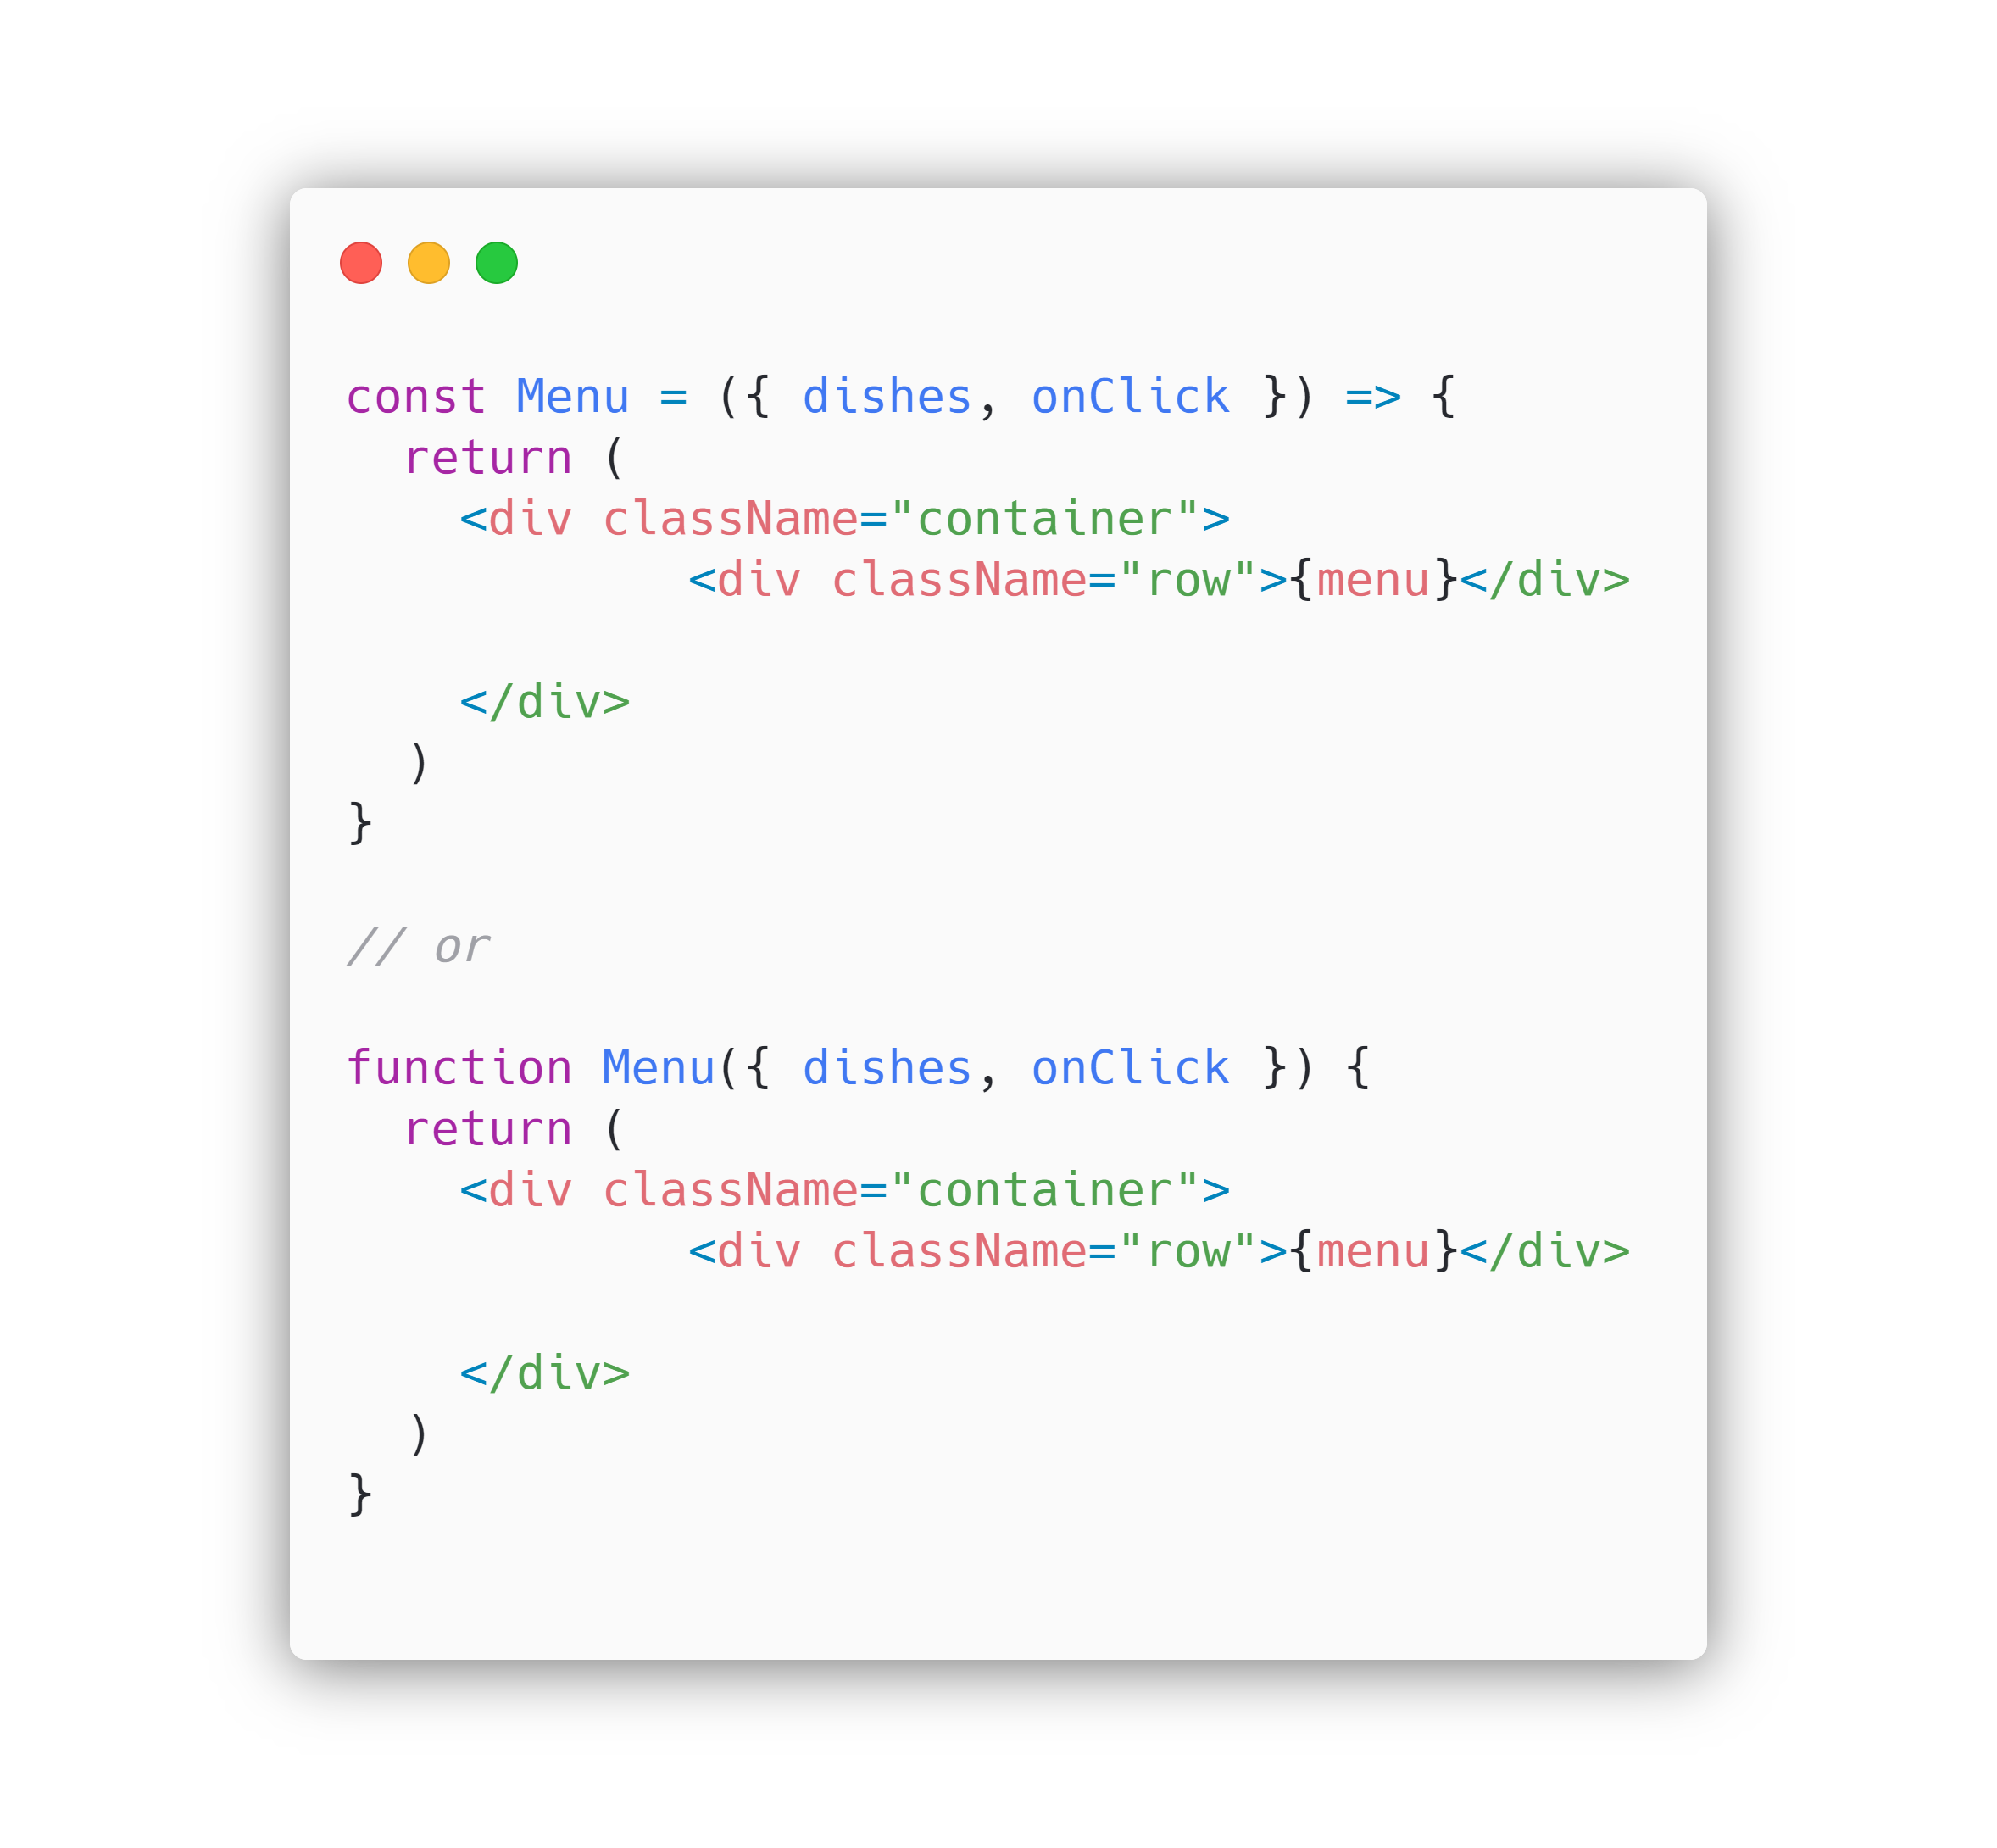
\includegraphics[width=\textwidth]{assets/class-vs-functional.png}
    \caption{Ways to define a functional components as function or arrow function}
\end{figure}

In React 16.8 it was introduced React Hooks to use lifecycle hooks also in functional component. This topic is not covered in courses, but will be discussed in the appendix of this document.

\subsubsection*{Document Object Model}
In the browser there is an object called \texttt{Browser DOM} (Document Object Model) and is the representation of the structure and data of a webpage. React uses a lightweight version of DOM called \texttt{Virtual DOM}, which uses an in-memory tree data structure of plain JavaScript objects, is extremely fast to manipulate compared to browser DOM and is fully recreated on every setState. 

There is a diffing algorithm that detect which nodes are changed and updates the only the minimum number of components in the sub-tree that is updated.

\subsubsection*{React Router}
React Router gives the ability to navigate between views using links. It's a module that need to be additionally installed into the React application called \texttt{react-router-dom}. It is a collection of navigational components that enable navigation among views and support a browser-based bookmarkable URLs to navigate in the web app. It is also possible to pass optional parameters.
This dependency allows you to use the \textit{<BrowserRouter>} tag, which enables navigation between multiple pages.
There is also the possibility to use \textit{<Route>} to specify the path to a page or component, or \textit{<Switch>} to group several routers and route the page according to state (like any switch).
Navigation is possible using \textit{<Link>} or \textit{<NavLink>}.

\subsubsection*{Parameters}
It is possible to pass parameters through the URL and pass it to the view, for example \textit{/menu/42} can be rendered in the view mapped to \textit{/menu} with an input parameter \textit{42}.

\subsubsection*{Forms}
In React there are two types of forms: controlled or unconttrolled.
Controlled forms are directly and bidirectionally tied to the state and every state mutation is associated with an handler.

An unconttrolled form is not tied to the state but holds the values internally in the DOM. It is possible to retrieve data, for example when sending information to a REST API, and does not need to have an handler for every state updte.


\subsection*{MVC Framework}
A Model-View-Controller is an architectural pattern commonly used to allow reusable components, isolate logic from user interface and permit indipendent development, testing and maintenance. 
The \textit{Model} part is normally used to manage behaviour and data, respond to requests about state or instruction to change state and notify the view when there is a change in the state.
The \textit{View} is used to present the information to the user in a user face.
A \textit{Controller} receive the input from the users, instructs the model on which action to perform and initiates a response.

React is not a full MVC framework (or its descendent Model-View View-Model), it only provides the presentation logic. The model and controller can be developed independently form the View using React.

\subsection*{Flux and Redux}
The Flux architecture is an alternative to the MVC approach. It is an unidirectional data flow, from an action to the view through a dispatcher and a store.
All updates have one unidirectional flow, the central unit is the store. If a view want to update the store it must use an action. It cannot update the store directly.
New action are propagated through the systems in response to user interaction and the dispatcher control all the changes that are made to the store.

\subsubsection*{Redux}
Redux is the place to store the state of the application and allow to have a consistent way to access it. Redux is widely adapted by the React community, but is not strictly connected to React itself. Redux make state mutations predictable.
The state is a single object and is the single source of truth, it is read only and the only way to change the state is through actions. Every change has to made with pure functions that takes the previous state and return a newly mutated one.
Using Redux is possible to implement logging utilities, api handling, undo/redo of a state and many other features.  
The store holds the current state value as a plain JavaScript object. There is some utilities provided from Redux to manage the store:
\begin{itemize}
    \item \textit{createStore} - method that allow to create a store with an initial state
    \item \textit{dispatch} - update the state with the provided action object
    \item \textit{subscribe} - accepts a callback function that will be run every time an action is dispatched
\end{itemize}

The bindings between React and Redux is possble using the package \textit{react-redux}. It will provide a function \textit{connect()} that generates a wrapper container that subscribes to the store. It takes 2 additional arguments:
\begin{itemize}
    \item \textit{mapStateToProps()} - called every time the store state changes. Return an object full of data with each field being a prop for the wrapped component
    \item \textit{mapDispatchToProps()} - eceives the dispatch() method and should return an object full of functions that us dispatch()
\end{itemize}

Surrounding the React App with a tag <Provider> allows to provide the store as an attribute and make it accessible as a singleton to all the connected components.

\subsubsection*{React-Redux-Form}
\textit{React-readux-form} is a versatile, fast and intuitive library for creating complex and performant forms in React using Redux, providing a collection of reducer and action creators. Form data are stored in a Redux store in a model. There is no need to do any creation or reducer function and it supports also validation for forms. It is suitable to use when there is need to persist form data across component mounting and unmounting.

\chapter*{Server-side Development with NodeJS, Express and MongoDB}

The second course taken introduced server-side application development with Node.js and its integration with the MongoDB database.

\section*{Node.js}

\subsubsection*{Node Modules}
A Node.js application is developed in modules, where each file corresponds to a module. The CommonJS\footnote{https://en.wikipedia.org/wiki/CommonJS} project defines this principle.


\begin{figure}[!ht]
    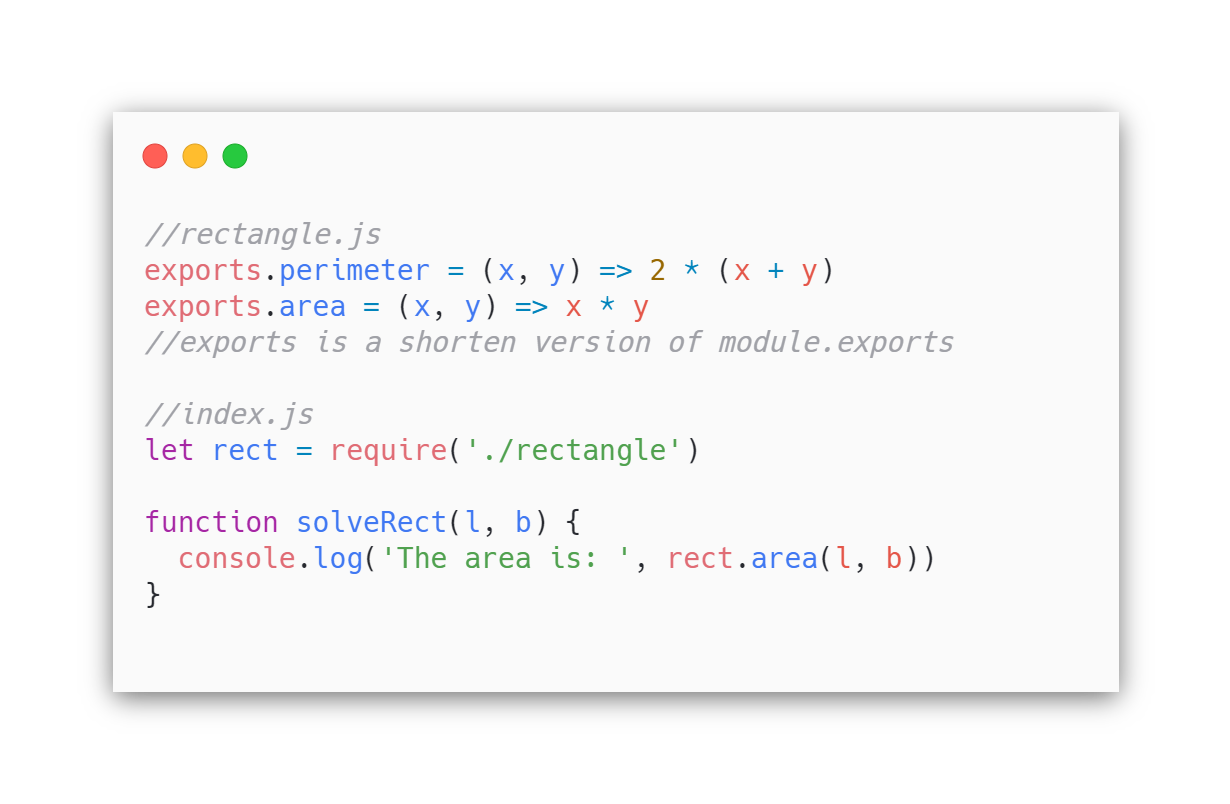
\includegraphics[width=\textwidth]{assets/modulenode.png}
    \caption{Example of a module and how to import}
    \label{fig:node-module}
\end{figure}

The module variable gives access to the current module definition in a file that can be exported using \textit{module.exports} or his shortand \textit{exports}.
The \textit{require} function is used to import a module.
There are several categories of module:
\begin{itemize}
    \item file-based modules
    \item core modules - part of Node's core like \textit{path}, \textit{fs}, or \textit{util}
    \item external modules - third-party modules installed using a package manager.
\end{itemize}


A module can be included using the \textit{require} function. A file-based module can be imported with \textit{require(module)} specifying the relative path to the file. It is enough for the core and external module to specify the module name, and Node will automatically look for external modules starting from \textit{node\_modules} folder up the hierarchy until the module is found.

\pagebreak

\subsubsection*{First-class functions and closures}
Node.js relies heavily on first-class functions and closures. A first-class function is a function that can be treated the same way as any other variable. For example, that can be passed as an argument to another function.
A closure is a function defined inside another function that has access to all the variables declared in the outer function (outer scope).
The inner function will continue to have access to the other variables from the outer scope even after the external function has returned.

\subsubsection*{Callback and Error handling}
Node.js is single-threaded, but at the same time, it can achieve a fast rate of completion of work. It is possible because of the judicious use of callbacks, the asynchronous execution of I/O requests, like file accesses or long-running processing that can be done independently behind the scenes.

Node.js continuously executes an event loop consisting of several phases:
\begin{itemize}
    \item timers - executes callbacks scheduled by \textit{setTimeout()} and \textit{setInterval}
    \item I/O callbacks - executes almost all calbacks with the exception od close callbacks and timers
    \item idle, prepare - internally used
    \item poll - retrieve I/O events, incoming connections, data, and others.
    \item check - \textit{setImmediate()} callbacks
    \item close callbacks - close callbacks like \textit{socket.on('close', ...)}
\end{itemize}
Each of these phases maintains its own separate queue, and the Node.js event loop picks up requests from each of these queues, and handles them. 

\subsection*{Networking}
Since network operations can cause unexpected delays and data is not instantaneously available, there is a need to write applications recognizing the asynchronous nature of communication. Network communications happens using the HTTP Client-Server communication protocol using the http module. Using this module is possible to create a server with \textit{http.createServer((res,req) +> {...})} and make it listen with \textit{server.listen(port,...)}.
The incoming messages are available through the \textit{req} parameter.

\subsection*{Express}
Express is the most popular third-party framework for building web servers. It is a fast, unopinionated, minimalist web framework for Node.js. It provides a robust set of features, and there are many third-party middlewares to extend functionality. An express application can be easily created using \textit{express-generator} through NPM.

A middleware provide a lot of plug-in functionality that can be used within your Express application. For example, \textit{morgan} is a plugin that can be used for logging

\subsubsection*{Router}
Express support routing URI through \textit{app.all, app.get, app.post, app.put} and \textit{app.delete} methods. This methods can be used to construct REST service:

\begin{center}
    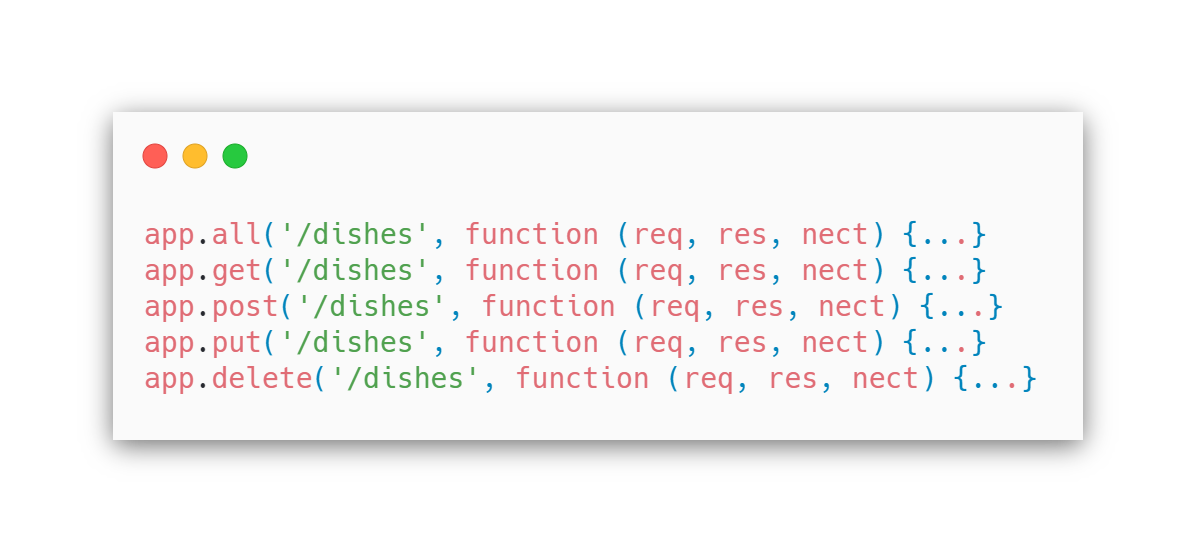
\includegraphics[width=0.8\textwidth]{assets/router.png}
\end{center}

It is possible to specify URI with parameters and to parse the body of a request using the \textit{body-parser} module.

There is also \textit{Express Router} for creaing mini-express application with routing abilities using \textit{myRouter = express.Router()} and then \textit{myRouter.route('/');}.

\subsection*{Authentication}
In Express, a request/response can pass through several middlewares that elaborate and propagate the modified request/response to the following middleware. For example, middleware could control if a request contains the necessary information to authenticate the user. If the user can be authenticated, the request can be propagated using the next() function; otherwise, it returns an error. 

\subsubsection*{Passport}
A node module that is an authentication middleware for Node.js. It is modular and flexible, it supports various strategies for authentication (local, openID, Oauth singgle sign-on, ...) and sessions.
Passport can be combined with Mongoose to simplify building login with username and password. It makes available Mongoose schema support for managing users, and it adds username, hash, and salt fields to store the username, the hashed password, and the salt value. It also provides additional methods to the User schema to support local authentication

\begin{center}
    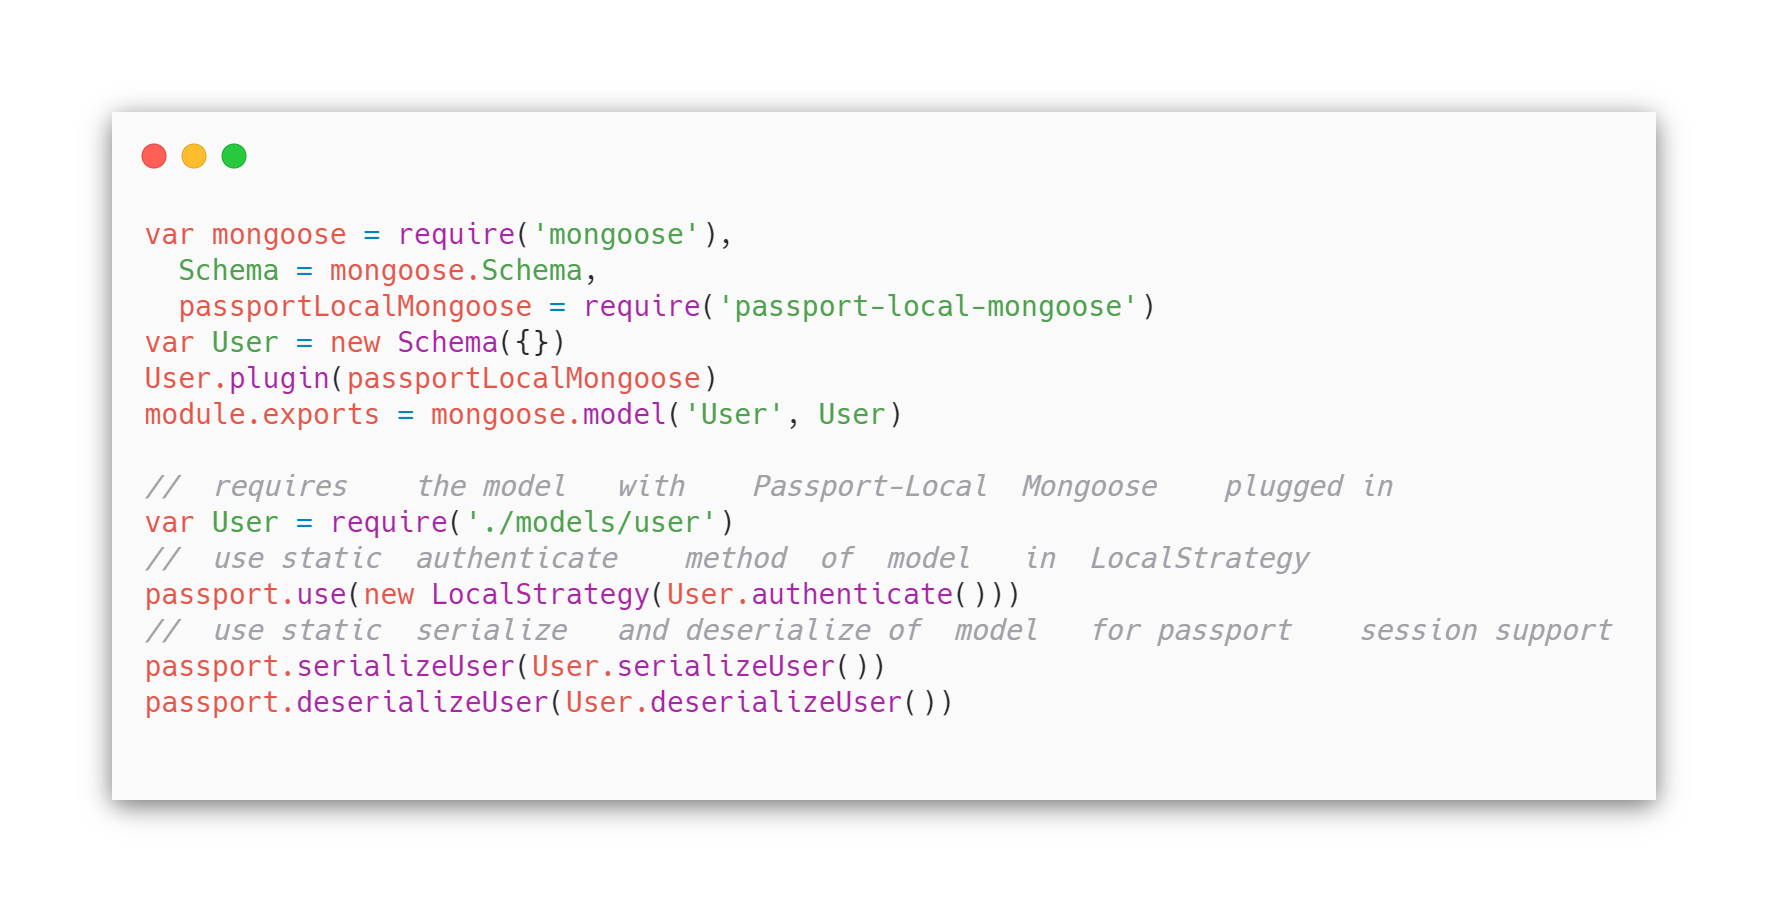
\includegraphics[width=0.8\textwidth]{assets/passport-mongoose.png}
    \label{fig:passport-mongoose}
\end{center}

Is it also possible to implement token-based authentication, especially if the server must be stateless and scalable or if the authentication should be shared between multiple servers. Token-based authentication helps to handle Cross-Origin resource sharing (CORS) problems and Cross-site request forgery.
The workflow is:
\begin{enumerate}
    \item User requests access with username and password
    \item Server validates credentials
    \item Server create a signed token and send it to the client (nothing is stored in the server)
    \item All subsequent requests from the client should include the token
    \item Server verifies the token and responds with data if validated
\end{enumerate}

To achieve token-based authentication in Express is possible to use jsonwebtoken and Passport-JWT modules. Passport-JWT creates and configures a new Passport strategy based on JWT authentication. It is possible to extract the JWT from an incoming request.

\subsubsection*{Sessions}
Sessions uses a combination of cookies and server-side storage to track users. A session is stored by default in a permanent memory server-side and it can be wiped out when the server restarts. It can be implemented using a middleware.

\begin{center}
    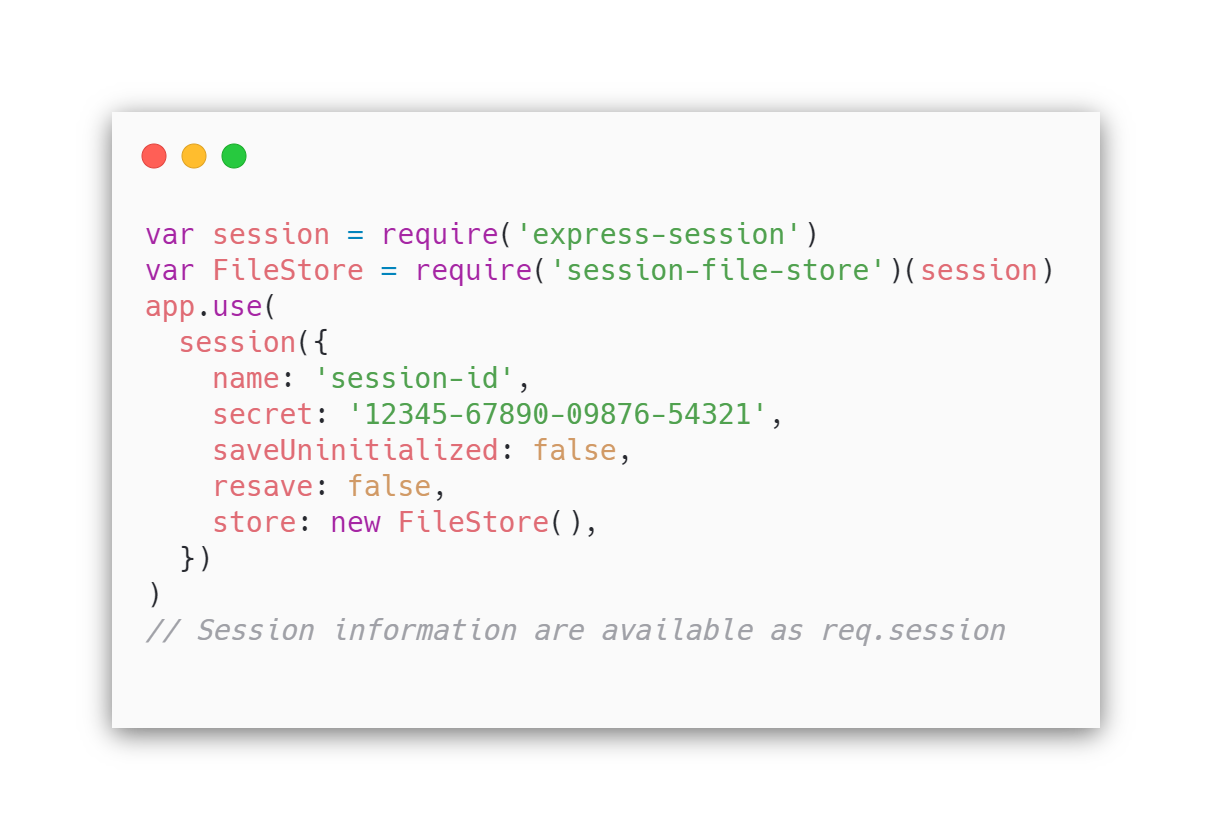
\includegraphics[width=0.8\textwidth]{assets/session.png}
    \label{fig:session}
\end{center}


\section*{MongoDB}

MongoDB is a document-based NoSQL DB. The document is a self-contained piece of information; it is possible to have a collection of documents, while a DB is a set of collections. A collection is a set of documents; a document is effectively a JSON file with some additional features. 
A NoSQL server can support multiple DBs. 
NoSQL's best features are scalability, availability, consistency, partition tolerance, and ease of deployment.

In MongoDB, documents are stored in a BSON (Binary JSON) format. It supports length prefix on each value, information about the field value type, and additional primitives type not supported by raw JSON like UTC date-time, raw binary, and ObjectID.

An ObjectID is a mandatory field \textit{\_id} created by MongoDB when a document is inserted.
MongoDB driver provides a high-level API for a Node application to interact with the MongoDB server for performing operations like connection, insertions, deletions, updates, and documents querying.

\subsection*{Mongoose ODM}
Mongoose ODM is a node module that gives a specific structure to documents and enforces the structure among all the applications. MongoDB stores data in the form of documents, but no structure is imposed on the document. Any document can be stored in any collection and relies on the developer's discipline to maintain the structure of the documents. MongoDB stores data in the form of documents, but no structure is imposed on the document. Any document can be stored in any collection and relies on the developer's discipline to maintain the structure of the documents.

\subsubsection*{Mongoose Schema}
It defines all the fields of the document and their types. It can do validation. Various schema types are String, number, date, buffer, boolean, mixed, ObjectID, and array. The schema is used to create a model function. Mongoose's schema types include String, Number, Date, Buffer, Boolean, Mixed, ObjectID, and Array. The Array schema type allows the creation of an array of sub-documents inside the document. Once a schema is defined, it is used in Mongoose to create a model function, which allows determining the structure for the documents in the database. Schemas can be nested to enable supporting embedded or sub-documents. 

\subsubsection*{Mongoose Population}
NoSQL databases like MongoDB usually do not explicitly support relations like the SQL databases. All documents are generally expected to be self-contained.
However, it is possible to store references to other documents within a document by using ObjectIds.

\begin{center}
    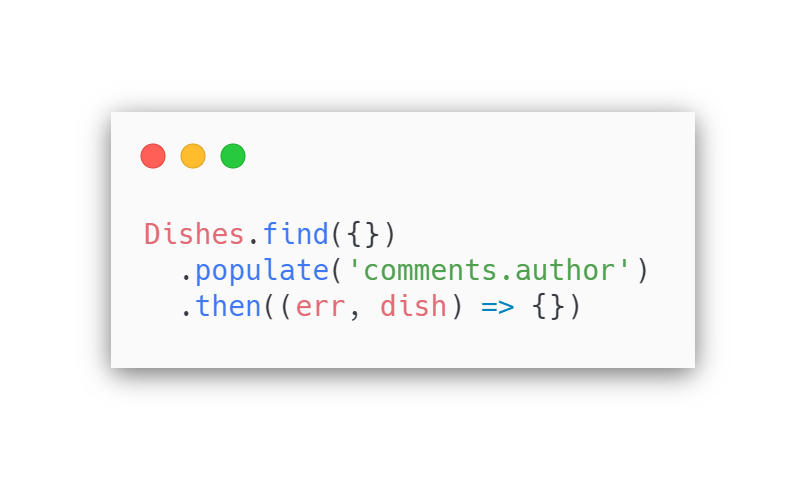
\includegraphics[width=0.8\textwidth]{assets/population.png}
\end{center}

Population automatically replaces specified paths within a document with documents from another collection using cross-reference with ObjectIds helps.
For example, an object 'comment' can have a rating, a comment, and an author.  It is possible to populate a Dish with a list of comments using Mongoose Population.

\chapter*{Conclusion}
This document summarizes the major and most important topics covered during these two courses. Within each course, there were exercises and assignments that were performed and completed and are freely available at this address: \url{https://github.com/gunghio-school/hk_react_course.git}

In addition, a personal project covering most of the topics was carried out in parallel.
It is a web app for booking articles for a butcher shop. The web app was developed using Next.js, a framework that combines frontend in React and backend in Node in a single application, and relies on a database in MongoDB.

The webapp can be accessed at \url{carne.gunghio.ch} after authentication using username \textit{neggio} and password \textit{matur}, while its source code is available at the following address: \url{https://github.com/OlmoBarberis/food-gunghio.git}.

In addition, all notes taken during the two courses are freely available at this address: \url{https://gunghio.notion.site/HK_Seminar-fcf71778e4bf4c2081368321089c6f1e}

% \bibliographystyle{unsrt}
% \nocite{*}
% \bibliography{bibliografia}

\end{document}
